\documentclass{article}
\usepackage[utf8]{inputenc}

\title{Assignment 5: EA}
\author{Luca Brena}
\date{December 2019}

\usepackage{natbib}
\usepackage{graphicx}
\graphicspath{ {./images/} }
\usepackage{amsmath}
\usepackage{enumitem}
\usepackage{subcaption}

\begin{document}

\maketitle

\section{Visualize test functions}
The contour plots of the test functions help a lot in the identification of the optimal values of the functions. The contour plots are shown in figure \ref{fig:image1}. In figure \ref{fig:image2} are plotted for both the test functions 100 uniformly sampled points evaluated with the test functions. The colours help to identify the optimum of the functions. In the case of the sphere function it's easy to see that in the optimum region is the one in wich the points are close to red. In the rastrigin case it's harder too see the optimum region because the function itself has many minimum points. Using the contour plot we can see that the optimum region is in the center of the function. This fact is confirmed by the scatter plot in which the point in the center of the plots are red. 

\begin{figure}[h]
	
	\begin{subfigure}{0.5\textwidth}
		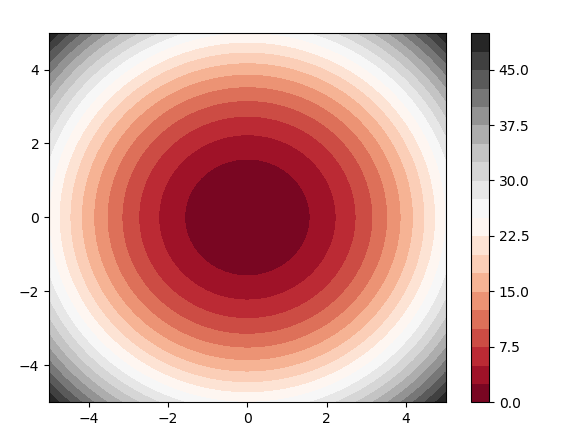
\includegraphics[width=0.9\linewidth, height=5cm]{sphere_contour.PNG} 
		\caption{2D contour plot for the sphere test function}
		\label{fig:subim1}
	\end{subfigure}
	\begin{subfigure}{0.5\textwidth}
		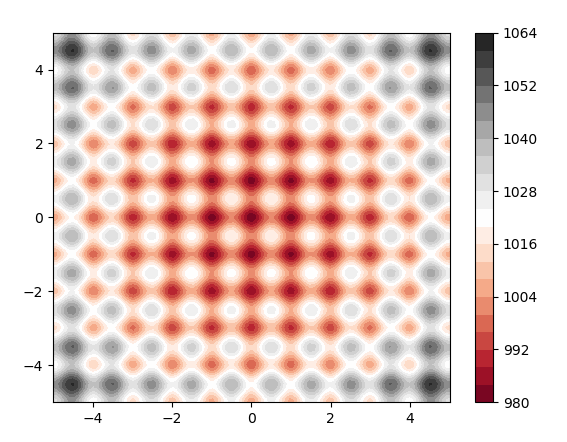
\includegraphics[width=0.9\linewidth, height=5cm]{rastrigin_contour.PNG}
		\caption{2D contour plot for the sphere test function}
		\label{fig:subim2}
	\end{subfigure}
	
	\caption{ }
	\label{fig:image1}
\end{figure}

\begin{figure}[h]
	
	\begin{subfigure}{0.5\textwidth}
		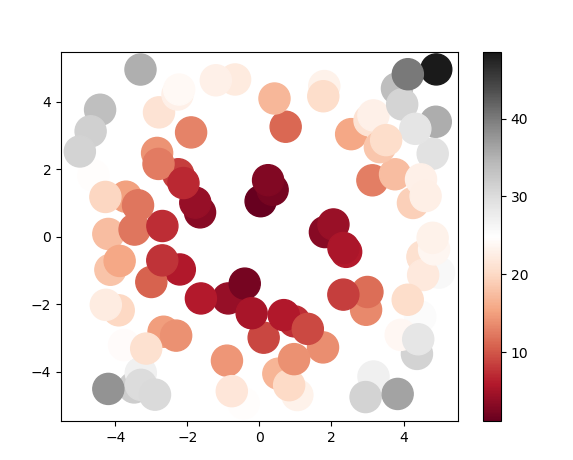
\includegraphics[width=0.9\linewidth, height=5cm]{sphere_dots.PNG} 
		\caption{2D plot of 100 samples evaluated with the sphere test function}
		\label{fig:subim3}
	\end{subfigure}
	\begin{subfigure}{0.5\textwidth}
		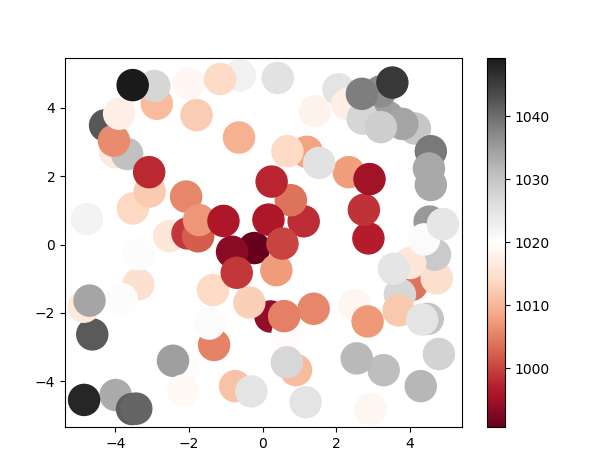
\includegraphics[width=0.9\linewidth, height=5cm]{rastrigin_dots.PNG}
		\caption{2D plot of 100 samples evaluated with the rastrigin test function}
		\label{fig:subim4}
	\end{subfigure}
	\caption{ }
	\label{fig:image2}
\end{figure}



\section{Cross-Entropy Method (CEM)}
The result of the \textit{CEM} are summarized in the tables \ref{tab:table1}, \ref{tab:table2}, \ref{tab:table1.1} and \ref{tab:table2.1}. The mean and the variance have been initializated following a uniform ditribution between -5 and 5 for the mean and from 0 to 5 for the variance. During the experiments i noticed a problem about the vanishing of the variance. So I added a small costant (0.001) during every generation. Best and worst fitness values for each generation, averaged on 3 runs of CEM are shown in figures \ref{fig:image3} and \ref{fig:image4}\\

\begin{table}[h]
\begin{tabular}{ |p{3cm}||p{3cm}|p{3cm}|p{3cm}|  }
	\hline
	\multicolumn{4}{|c|}{Number of samples: 100, Number of features: 100, Test function: sphere} \\
	\hline
    Number of generations& Elite set & Best Fitness & Worst Fitness\\
	\hline
	50   & 20    &89.6&   93.5\\
	100 &   20  & 72.7   &74.0\\
	1000 & 20 & 0.0&  0.0\\
	50    &50 & 70.6&  82.9\\
	100&   50  & 41.7& 44.1\\
	1000& 50  & 0.4   &0.5\\
	
	\hline
\end{tabular}
\caption{\label{tab:table1} }
\end{table}

\begin{table}[h]
\begin{tabular}{ |p{3cm}||p{3cm}|p{3cm}|p{3cm}|  }
	\hline
	\multicolumn{4}{|c|}{Number of samples: 1000, Number of features: 100, Test function: sphere} \\
	\hline
	Number of generations& Elite set & Best Fitness & Worst Fitness\\
	\hline
	50   & 200    &12.1&   14.4\\
	100 &   200  & 10.1  &10.1\\
	1000 & 200 & 0.1&  0.1\\
	50    &500 & 61.7&  82.2\\
	100&   500  & 20.3& 21.9\\
	1000& 500  & 0.0   &0.0\\
	
	\hline
\end{tabular}
\caption{\label{tab:table2} }
\end{table}

\begin{table}[h]
	\begin{tabular}{ |p{3cm}||p{3cm}|p{3cm}|p{3cm}|  }
		\hline
		\multicolumn{4}{|c|}{Number of samples: 100, Number of features: 100, Test function: rastrigin} \\
		\hline
		Number of generations& Elite set & Best Fitness & Worst Fitness\\
		\hline
		50   & 20    &158.0&   160.1\\
		100 &   20  & 270.6   &271.3\\
		1000 & 20 &9362.3&  9362.3\\
		50    &50 & 491.3& 807.7\\
		100&   50  & 478.6& 629.6\\
		1000& 50  &9256.0   &9256.0\\
		
		\hline
	\end{tabular}
	\caption{\label{tab:table1.1} }
\end{table}

\begin{table}[h]
	\begin{tabular}{ |p{3cm}||p{3cm}|p{3cm}|p{3cm}|  }
		\hline
		\multicolumn{4}{|c|}{Number of samples: 1000, Number of features: 100, Test function: rastrigin} \\
		\hline
		Number of generations& Elite set & Best Fitness & Worst Fitness\\
		\hline
		50   & 200    &301.1&   747.3\\
		100 &   200  & 310.5  &542.0\\
		1000 & 200 & 9186.6&  9186.6\\
		50    &500 & 469.1&  907.2\\
		100&   500  & 778.8& 1247.1\\
		1000& 500  & 9120.0  &9120.0\\
		
		\hline
	\end{tabular}
	\caption{\label{tab:table2.1} }
\end{table}

\begin{figure}
	\centering
	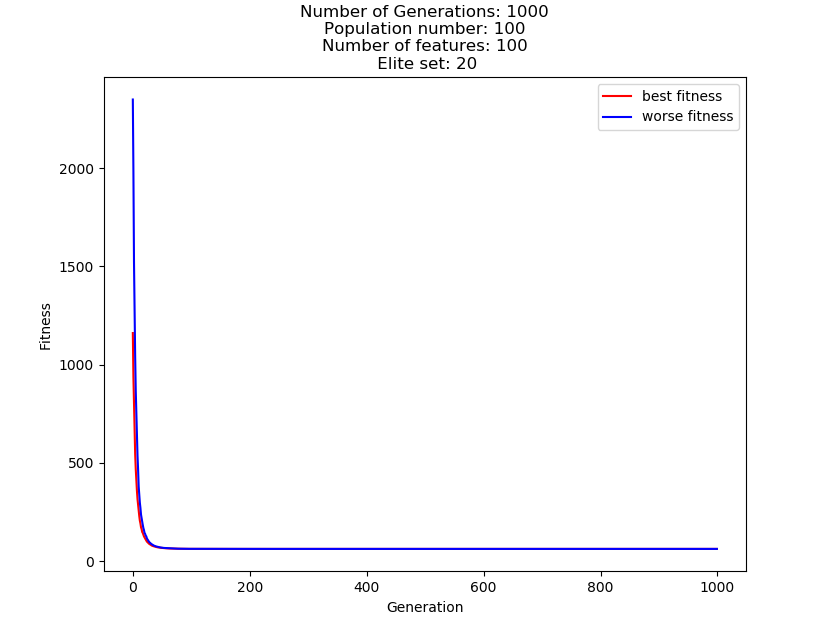
\includegraphics[width=\textwidth]{CEM_d_sphere.png}
	\caption{ Best and worst fitness values for each generation, averaged on 3 runs of CEM for the sphere function.}
	\label{fig:image3}
\end{figure}

\begin{figure}
	\centering
	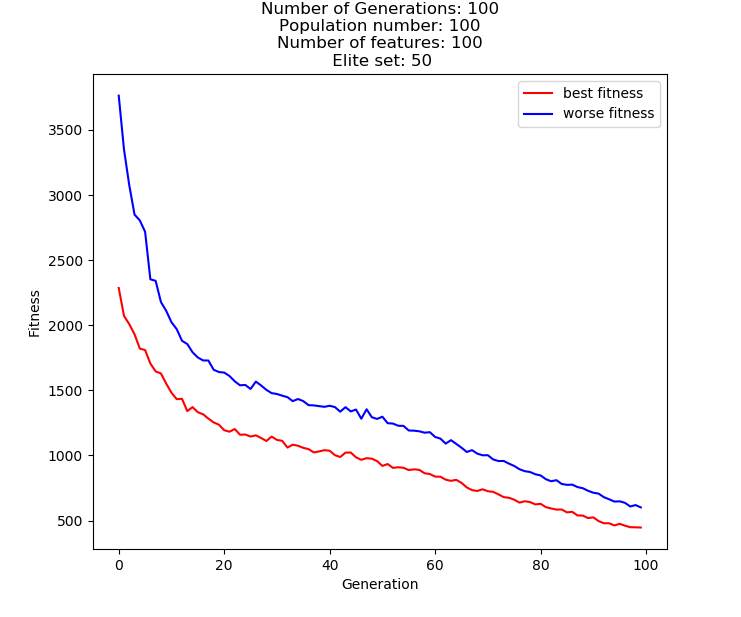
\includegraphics[width=\textwidth]{CEM_d_rastrigin.png}
	\caption{ Best and worst fitness values for each generation, averaged on 3 runs of CEM for the rastrigin function.}
	\label{fig:image4}
\end{figure}

\section{Natural Evolution Strategy (NES)}
The result of  \textit{NES} are summarized in the tables \ref{tab:table3}, \ref{tab:table4}, \ref{tab:table3.1} and \ref{tab:table4.1}  The mean and the variance have been initializated following a uniform ditribution between -5 and 5 for both means and covariance matrix. Best and worst fitness values for each generation, averaged on 3 runs of NES are shown in figures \ref{fig:image5}\\\\

\begin{table}[h]
\begin{tabular}{ |p{3cm}||p{3cm}|p{3cm}|p{3cm}|  }
	\hline
	\multicolumn{4}{|c|}{Number of samples: 100,  Number of features: 100, Test function: sphere} \\
	\hline
	Number of generations& Learning Ratio & Best Fitness & Worst Fitness\\
	\hline
	50   & 0.01    &error&  error\\
	100 &   0.01  & error   & error\\
	1000 & 0.01 & error&  error\\
	50    &0.001 & 13.3& 64.0\\
	100&   0.001  & error& error\\
	1000& 0.001  & error   &error\\
	
	\hline
\end{tabular} 
\caption{\label{tab:table3} }
\end{table}


\begin{table}[h]
\begin{tabular}{ |p{3cm}||p{3cm}|p{3cm}|p{3cm}|  }
	\hline
	\multicolumn{4}{|c|}{Number of samples: 1000,  Number of features: 100, Test function: sphere} \\
	\hline
	Number of generations& Learning Ratio & Best Fitness & Worst Fitness\\
	\hline
	50   & 0.01    & error & error\\
	100 &   0.01  & 92.8   &223.1\\
	1000 & 0.01 & error&  error\\
	50    &0.001 & 598.2& 1389.1\\
	100&   0.001  &415.0& 1019.8\\
	1000& 0.001  & 286.0   & 784.7\\
	
	\hline
\end{tabular}
\caption{\label{tab:table4} }
\end{table}


\begin{table}[h]
	\begin{tabular}{ |p{3cm}||p{3cm}|p{3cm}|p{3cm}|  }
		\hline
		\multicolumn{4}{|c|}{Number of samples: 100,  Number of features: 100, Test function: rastrigin} \\
		\hline
		Number of generations& Learning Ratio & Best Fitness & Worst Fitness\\
		\hline
		50   & 0.01    &error&  error\\
		100 &   0.01  & error   & error\\
		1000 & 0.01 & error&  error\\
		50    &0.001 & error& error\\
		100&   0.001  & error& error\\
		1000& 0.001  & error   &error\\
		
		\hline
	\end{tabular} 
	\caption{\label{tab:table3.1} }
\end{table}


\begin{table}[h]
	\begin{tabular}{ |p{3cm}||p{3cm}|p{3cm}|p{3cm}|  }
		\hline
		\multicolumn{4}{|c|}{Number of samples: 1000,  Number of features: 100, Test function: sphere} \\
		\hline
		Number of generations& Learning Ratio & Best Fitness & Worst Fitness\\
		\hline
		50   & 0.01    & error & error\\
		100 &   0.01  & error   & error\\
		1000 & 0.01 & error&  error\\
		50    &0.001 & error& error\\
		100&   0.001  & error & error\\
		1000& 0.001  & error   & error\\
		
		\hline
	\end{tabular}
	\caption{\label{tab:table4.1} }
\end{table}

\begin{figure}
	\centering
	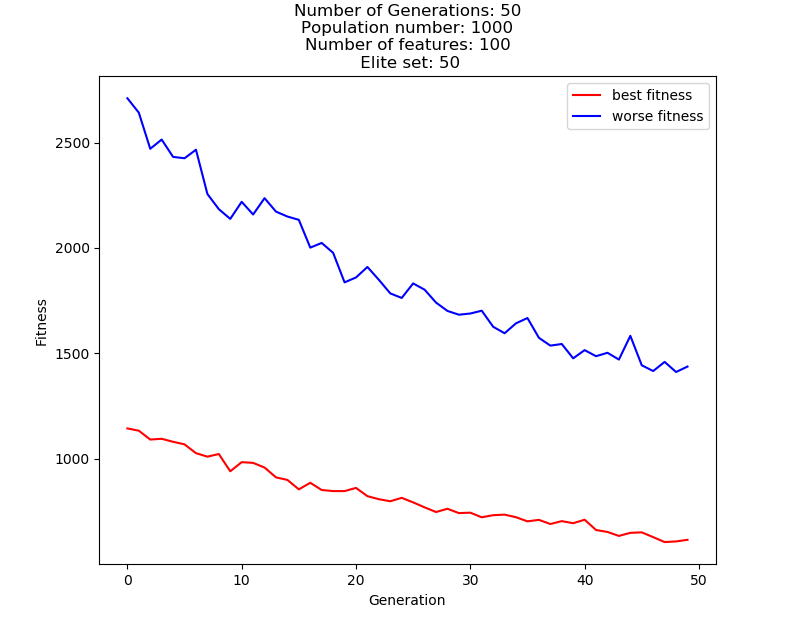
\includegraphics[width=\textwidth]{NES_d_sphere.png}
	\caption{ Best and worst fitness values for each generation, averaged on 3 runs of NES for the sphere function.}
	\label{fig:image5}
\end{figure}


\section{Covariance Matrix Adaptation Evolution Strategy (CMA-ES)}
The result of  \textit{CMAES} are summarized in the table \ref{tab:table5},\ref{tab:table6}, \ref{tab:table5.1}, \ref{tab:table6.1}.The mean and the variance have been initializated following a uniform ditribution between -5 and 5 for both means and covariance matrix. For this case i used only 20 features because every run of the algorithm takes several minutes with higher dimensional spaces.  Best and worst fitness values for each generation, averaged on 3 runs of CMAES are shown in figures \ref{fig:image7},  \ref{fig:image8} \\

\begin{table}[h]
\begin{tabular}{ |p{3cm}||p{3cm}|p{3cm}|p{3cm}|  }
	\hline
	\multicolumn{4}{|c|}{Number of samples: 100,  Number of features: 20, Test function: sphere} \\
	\hline
	Number of generations& Elite set & Best Fitness & Worst Fitness\\
	\hline
	50   & 20    &26.1& 26.1\\
	100 &   20  & 49.1   & 49.1\\
	1000 & 20 & 78.9&  78.9\\
	50    &50 & 39.4& 39.4\\
	100&   50  &43.9& 43.9\\
	1000& 50  & 37.9   &37.9\\
	
	\hline
\end{tabular} 
\caption{\label{tab:table5} }
\end{table}

\begin{table}[h]
	\begin{tabular}{ |p{3cm}||p{3cm}|p{3cm}|p{3cm}|  }
		\hline
		\multicolumn{4}{|c|}{Number of samples: 1000,  Number of features: 20, Test function: sphere} \\
		\hline
		Number of generations& Elite set & Best Fitness & Worst Fitness\\
		\hline
		50   & 200    &3.4&3.4\\
		100 &   200  & 0.0   & 0.0\\
		1000 & 200 & 0.0& 0.0\\
		50    &500 & 0.0& 0.0\\
		100&   500  & 0.0& 0.0\\
		1000& 500  & 0.0   & 0.0\\
		
		\hline
	\end{tabular} 
	\caption{\label{tab:table6} }
\end{table}


\begin{table}[h]
	\begin{tabular}{ |p{3cm}||p{3cm}|p{3cm}|p{3cm}|  }
		\hline
		\multicolumn{4}{|c|}{Number of samples: 100,  Number of features: 20, Test function: rastrigin} \\
		\hline
		Number of generations& Elite set & Best Fitness & Worst Fitness\\
		\hline
		50   & 20    &437.8& 438.1\\
		100 &   20  & 916.5   &916.5\\
		1000 & 20 &9933.1&  9933.1\\
		50    &50 & 428.2& 439.3\\
		100&   50  943.6& 943.6\\
		1000& 50  &9937.0   &9937.0\\
		
		\hline
	\end{tabular} 
	\caption{\label{tab:table5.1} }
\end{table}

\begin{table}[h]
	\begin{tabular}{ |p{3cm}||p{3cm}|p{3cm}|p{3cm}|  }
		\hline
		\multicolumn{4}{|c|}{Number of samples: 1000,  Number of features: 20, Test function: rastrigin} \\
		\hline
		Number of generations& Elite set & Best Fitness & Worst Fitness\\
		\hline
		50   & 200    &319.7&320.6\\
		100 &   200  & 816.9   & 816.9\\
		1000 & 200 &9811.2& 9811.2\\
		50    &500 & 392.2& 574.6\\
		100&   500  &816.8& 845.2\\
		1000& 500  & error  & error\\
		
		\hline
	\end{tabular} 
	\caption{\label{tab:table6.1} }
\end{table}

\begin{figure}
	\centering
	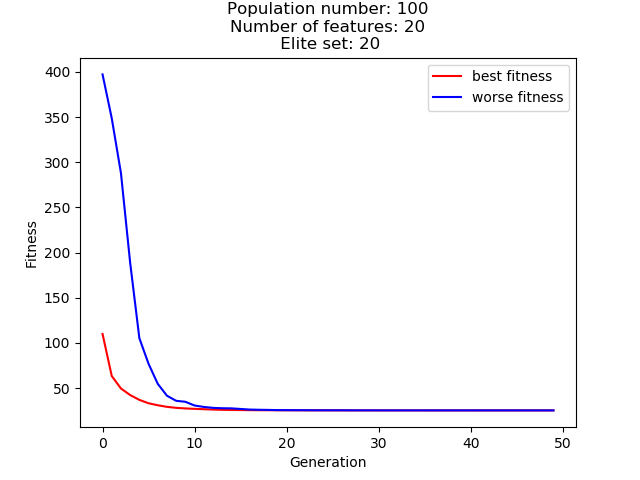
\includegraphics[width=\textwidth]{CMA_d_sphere.png}
	\caption{ Best and worst fitness values for each generation, averaged on 3 runs of CMA for the sphere function.}
	\label{fig:image7}
\end{figure}

\begin{figure}
	\centering
	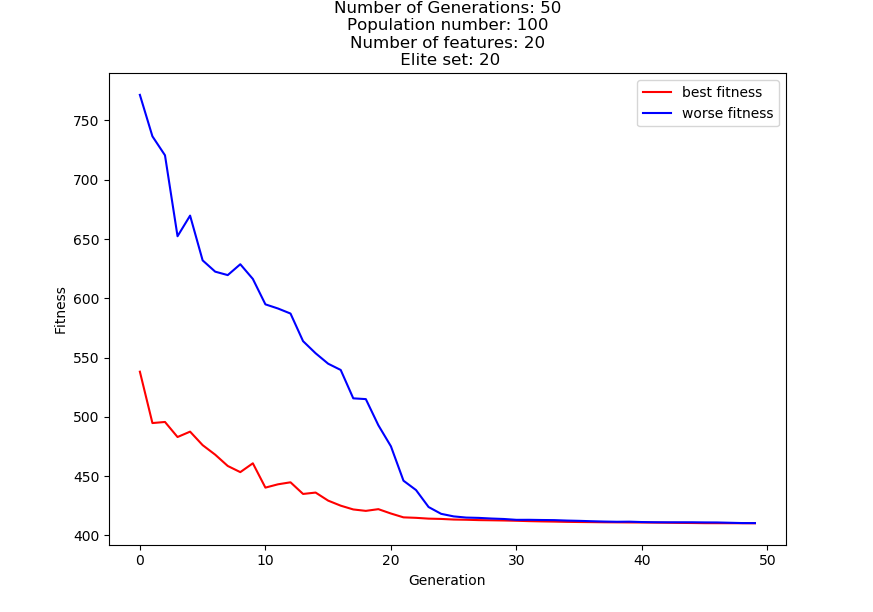
\includegraphics[width=\textwidth]{CMA_d_rastrigin.png}
	\caption{ Best and worst fitness values for each generation, averaged on 3 runs of CMA for the sphere function.}
	\label{fig:image8}
\end{figure}




\end{document}
